\documentclass[11pt]{article}
\usepackage{fullpage}
\usepackage{titlesec}
\usepackage{times}
\usepackage{graphicx}
\usepackage{amsmath}
\usepackage{url}
\usepackage{hyperref}

\usepackage{cite}


\titlelabel{\thetitle.\quad}

\title{CS252 Assignment-1}
\author{Arnab Bhattacharya}
\date{\today}
\begin{document}
\maketitle

\section {Introduction}
\label{sec:intro}
In this document , the approach to the previous phases has been explained along with their detailed explanation.The methods used in all the phases has been described in the respective sections.
Following are the few of the references used by: 
 ~\cite{google}
 ~\cite{cs251}
 ~\cite{perl}
 ~\cite{sql}


\section{Phase-1 : Octave}
\label{sec:ph1}
The file phase1.m implements a {\bf Octave} script to solve the problem. First , we created two matrix to store the roll number of the 100 students and the other matrix to store the data of those 100 students. The roll number's were generated using the random function. After that ,we rounded off the roll numbers and then sorted it. Courses and marks where allotted using the random function and uniqueness was achieved by comparing the values with the previous entities. All the data was written in "phase1.out" using "csvwrite" command.

\section{Phase-2 : Perl}
\label{sec:ph2}
The perl script phase2.pl creates a table named marks and names in a Mysql Database. The table "marks" has five columns : roll ,  course , project , assignment and marks with roll and course as the primary key. It also creates another table names in the same database with two columns : names and roll numbers
with roll as the primary key. It then inserts all the names from the file names.txt along with the roll numbers from phase1.out.
The name corresponding to the ith line in the file has the ith roll number in ascending order.The data in table marks was filled entirely from phase1.out.
 
 \section{Phase-3 : Mysql}
 \label{sec:ph3}
 The Mysql script adds two columns named grade and total using Alter table command. The total has the sum of assignment,project and exam for each course. Grade is decided according to the formula:\\
 $$
Grade = 
\begin{cases}
A* & total\geq95\% \\
A & 80\% \leq total < 95\% \\
B & 60\% \leq total < 80\% \\
C & 45\% \leq total < 60\% \\
D & 30\% \leq total < 45\% \\
F & total < 30\% \\
\end{cases}
$$\\
The number of students for each grade category in each course was saved in a file as phase3.out. The entire MySQL script was named as phase3.sql.

\section{Phase-4 : Formatting(Perl)}
\label{sec:ph4}
The script is written in perl and it prepares the data in a format that the GnuPlot script of phase-5 can consume. It just makes arrays for each grade and then data is pushed accordingly in phase4.out.

\section{Phase-5 : Gnuplot }
\label{sec:ph5}
The script is written in gnuplot and it makes a histogram which plots the number of students  in each grade per course.
\begin{figure}[!hb]
\centering
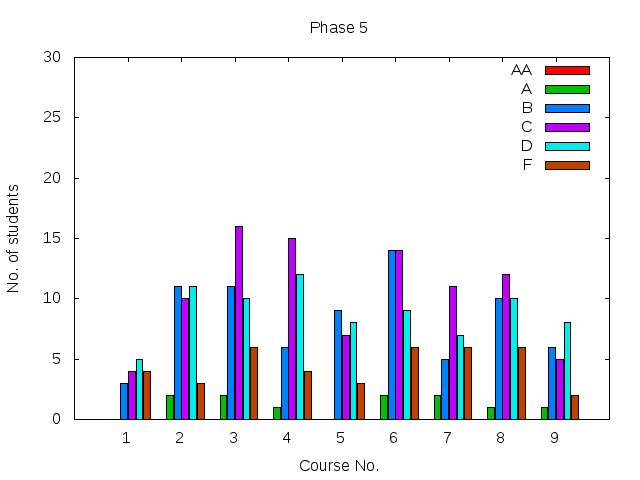
\includegraphics[scale=0.5]{phase5.png}
\caption{Phase 5}
\end{figure}
 
 \section{Phase-6 : Latex}
 \label{sec:ph6}
 The phase6.tex and phase6.bib after compiling gives this file  that describes the entire process so far including how the marks for students are generated, how the grades are assigned, etc. It contains tables, figures (the plot produced in phase-5), equations, referencing, etc.
 
 \section{Phase-7 : Bash}
 \label{sec:ph7}
 The bash scripts produces a ranked list of all students according to their total marks for every course. It extracts the raw data out from the MySQL table marks without sorting the students based on total.The aim was to segregate, sort and find the ranks using Bash. We used auxiliary Bash tools such as Grep, Sed, Awk, etc to produce a single output file phase7.out that contains the ranked lists of the 9 courses in order.
 
 \section{Phase-8 : Automation(Bash)}
 \label{sec:ph8}
 The bash script connects the first 7 phases together by making a single file to run all the 7 phases together. This file  contains the commands of how to run each phase, what it inputs, what it outputs, etc.
 

\bibliographystyle{plain}
\bibliography{phase6.bib}
\end{document}
